\chapter{Questionnaire}\label{appendix:questionnaire}
\myappendices{Appendix \ref{appendix:questionnaire} {Questionnaire}}

\begin{figure}[h]
   \centerline{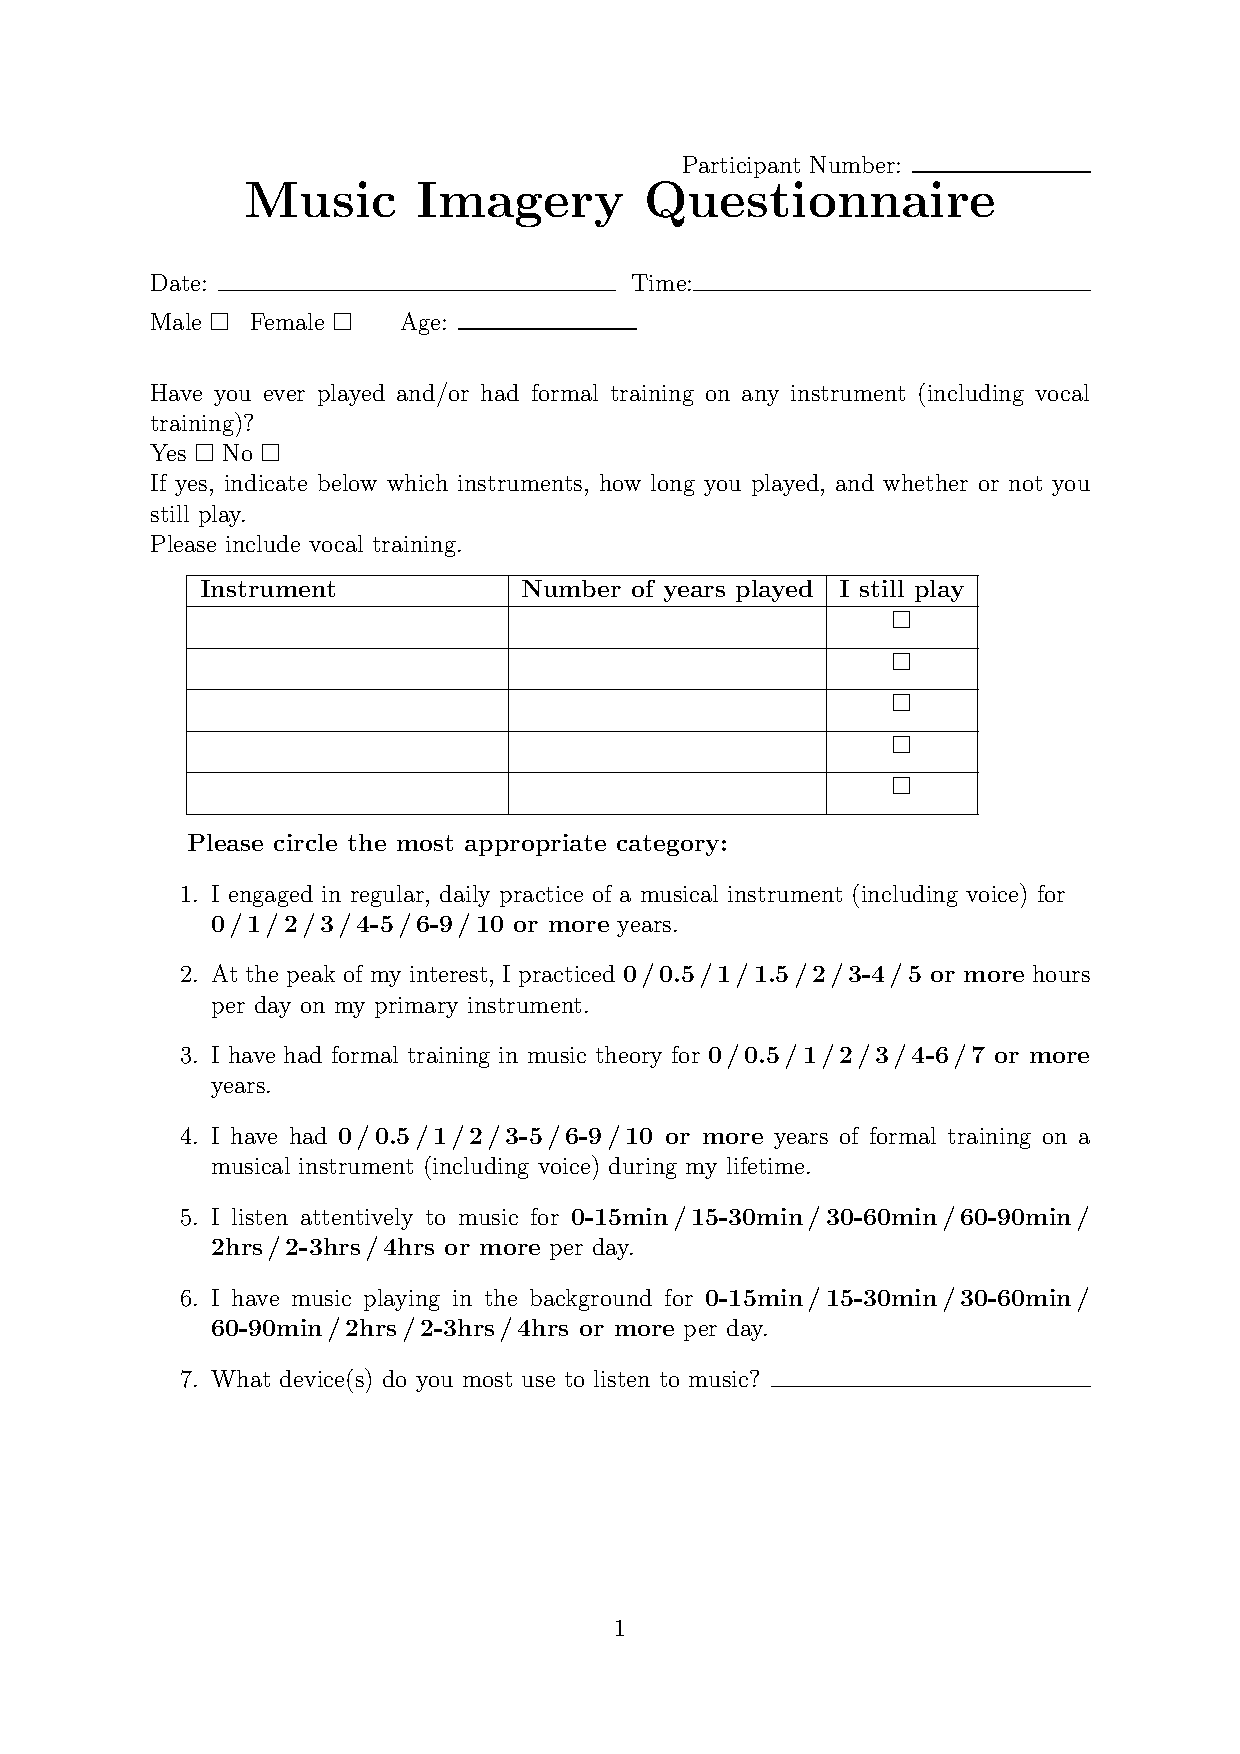
\includegraphics[page=1,scale=0.75,trim={0.75in 2in 0.75in 1in},clip]{Figures/questionnaire.pdf}}
\end{figure}

% this is shorter but does not generate page numbers and headers - they get taken from the included pdf
%\includepdf[pages={2-3},scale=0.75,trim={0in 1in 0in 0.5in},clip]{Figures/questionnaire.pdf}

%% you only have two pages! so do brute force, one page at a time, same scale as before
\begin{figure}[h]
   \centerline{\includegraphics[page=2,scale=0.75,trim={0in 1in 0in 0.5in},clip]{Figures/questionnaire.pdf}}
\end{figure}

\begin{figure}[h]
   \centerline{\includegraphics[page=3,scale=0.75,trim={0in 1in 0in 0.5in},clip]{Figures/questionnaire.pdf}}
\end{figure}